\documentclass{article}
\usepackage{graphicx}
\usepackage{nameref}
\usepackage{hyperref}
\usepackage{fontspec}
\setmainfont{Arial}
\setlength{\parindent}{0pt}
\setlength{\parskip}{5pt}
\begin{document}

\section{Summary}
Reduce translation costs in multilanguage publishing.

\begin{itemize}
\item human encodes a text
\item software generates human languages
\end{itemize}

Business uses the technology through a translation agency.


\subsection{Reduce translation costs: an example}

Task: translate a document to 10 languages.

\begin{itemize}
\item Cost before: 10.000€
\item Cost after: 2.000€
\item Saving: 8.000€
\end{itemize}

\paragraph{Traditional approach}

\begin{itemize}
\item Translate to 10 languages, 1.000€ per translation
\item Cost: 10.000€
\end{itemize}

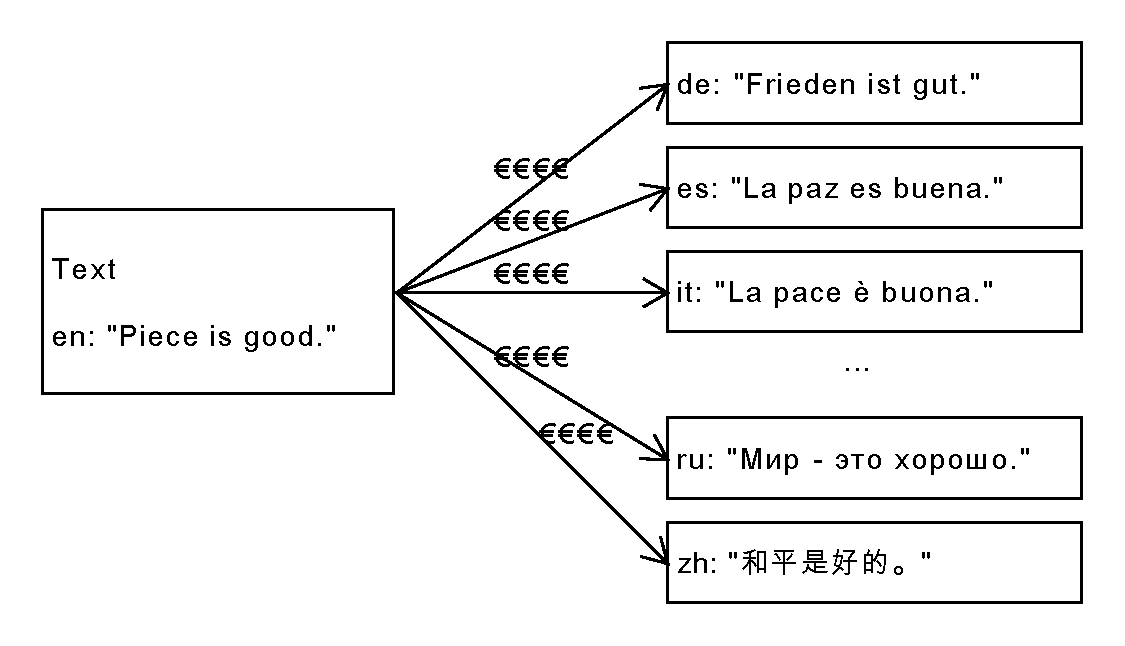
\includegraphics[scale=0.4]{dia/user-view-current-world.pdf}

\paragraph{New approach}

\begin{itemize}
\item Encode the document: 2.000€
\item Generate 10 language versions: doesn't cost anything
\item Cost: 2.000€
\end{itemize}

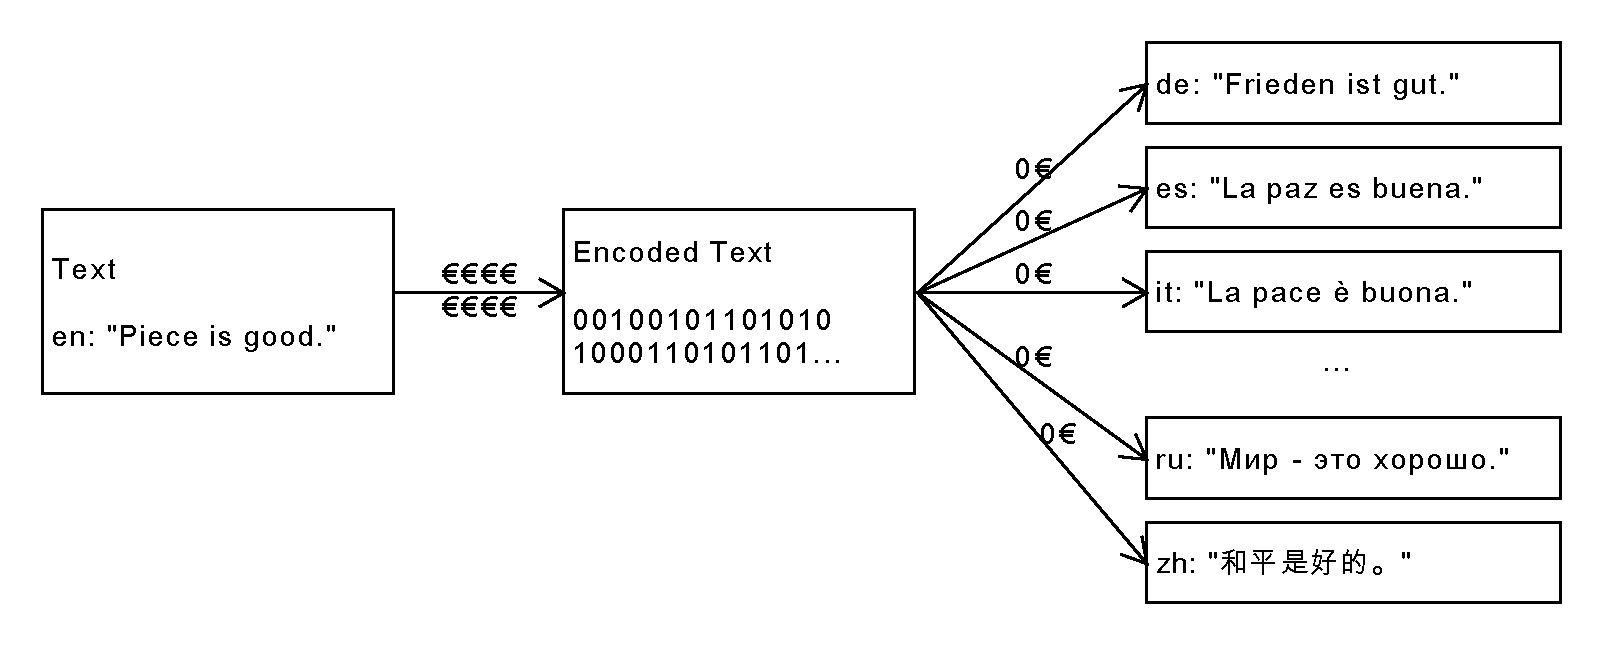
\includegraphics[scale=0.4]{dia/user-view-tokimani.pdf}


\section{Technology}

Existing attempts: full automation

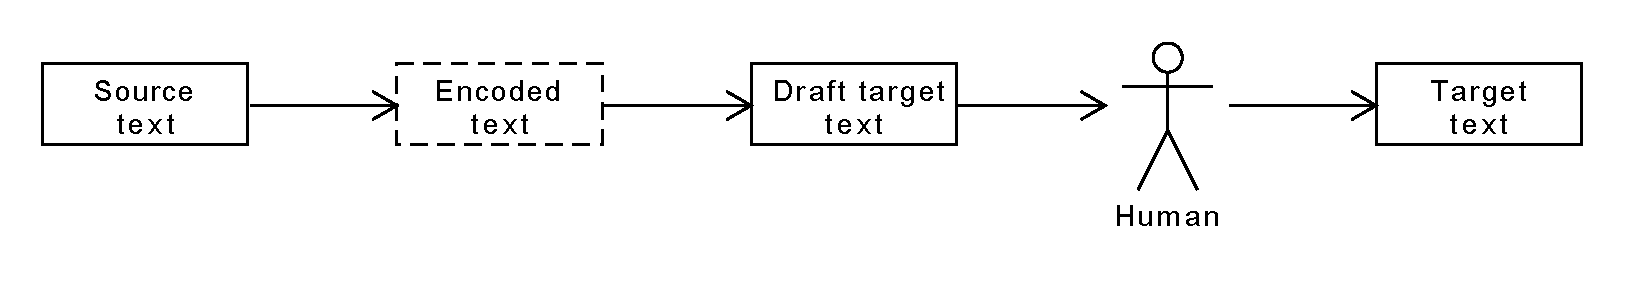
\includegraphics[scale=0.5]{dia/how-current-world.pdf}

Our approach: human in the loop

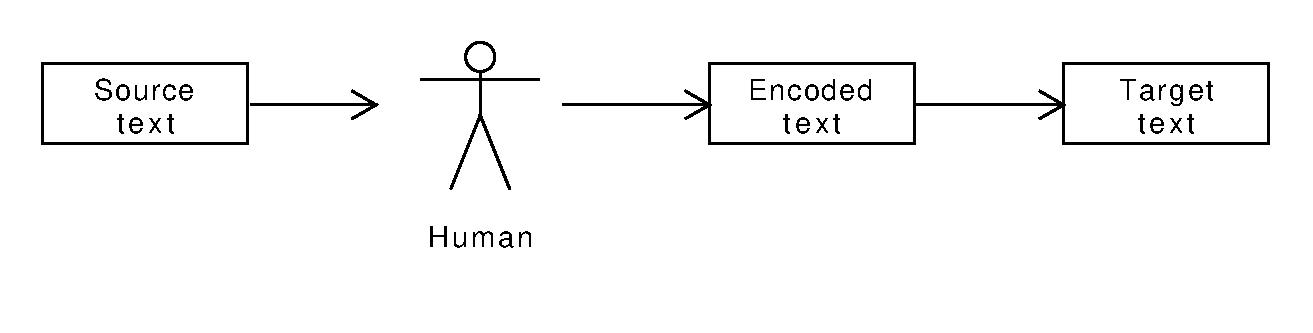
\includegraphics[scale=0.5]{dia/how-tokimani.pdf}

The difference:
\begin{itemize}
\item encoding is made by a human
\item encoded text is human-friendly (for a trained human)
\end{itemize}

\subsection{Alternative technologies}

Must-have

\begin{itemize}
\item retain the meaning
\item publish immediately
\end{itemize}

\subsection{Why it doesn't exist already}

My hypothesis is: the step "source text to encoded text" can't be automated.

\subsubsection{Fall 1: research}

\begin{itemize}
\item Business has an idea "one source to many targets", likely with the word "automatically".
\item Business ask an university for joint work.
\item Our approach brings nothing scientific new. It leads to no papers. No papers means the end of an academic carier.
\item A researcher subconciously discards our approach even before it comes into mind.
\end{itemize}

\subsubsection{Fall 2: human-first bias}

In related areas, there are successful projects, in which "source text" is restricted by rules, so that "source text" becomes also "encoded text". The keyword is "controlled English".

We go a step further. We declare that being a hauman language is a downside, not a benefit.

\begin{itemize}
\item Having code instead of text is custom-breaking. People don't like changing habits.
\item "Source text" is a front door to a system. A human languages hides complexity elsewhere and gives impresstion that the system is easy.
\end{itemize}


\section{Minimal value product}

To be presented at an user meeting.

\begin{itemize}
\item Audience proposes a phrase conforming to [ASD-STE]
\item The presenter encodes the phrase
\item The system generates English, German, Russian and Spanish
\end{itemize}

\subsection{Milestones}\label{milestones}

We rely on:

\begin{itemize}
\item Grammatical Framework [GF], [GF-TALK] and its GF-RGL [GF-RGL] library for multilanguage generation.
\item Lojban [LOJBAN] as inspiration for text encoding.
\end{itemize}

Steps:

\begin{itemize}
\item Done: to learn GF and GF-RGL: describe a small constructed language Toki Pona [TOKIPONA] in GF: [GF-TOKIPONA].
\item Extract examples from "Simplified Technical English" [ASD-STE], encode them in GF-RGL. Use the examples as the ground truth.
\item Learn Lojban, translate the examples to Lojban.
\item Write a converter Lojban to GF-RGL for the examples.
\item Derive CODENAME from Lojban experiments, with a converter from CODENAME to GF-RGL.
\item Create a tool to manage the dictionary.
\item Make Generated texts in English, German, Russian and Spanish good.
\item Profit.
\end{itemize}

References:

\begin{itemize}
\item ASD-STE. ASD Simplified Technical English, \url{http://www.asd-ste100.org/}
\item GF. Grammatical Framework, \url{https://www.grammaticalframework.org/}
\item GF-RGL. GF Resource Grammar Library (RGL), \url{https://github.com/GrammaticalFramework/gf-rgl}
\item GF-TALK. Grammatical Framework: Formalizing the Grammars of the World, \url{https://www.youtube.com/watch?v=x1LFbDQhbso}
\item GF-TOKIPONA. Describe Toki Pona using Grammatical Framework, \url{https://github.com/olpa/gf-tokipona}
\item LOJBAN. Lojban, \url{https://www.lojban.org/}
\item TOKIPONA. Toki Pona, \url{https://tokipona.org/}
\end{itemize}


\section{Sample promotion}\label{promotion}

We can start promoting the product and build the client base even without a MVP. The prerequisite is that the following phrase (from the specification ASD-STE100, issue 6, page 70) works in the system:

>> Each engine has a CSD to operate the AC generator at a constant speed of 8000 rpm. Differences in engine rpm and generator load have no effect on this constant speed. <<

\subsection{Sample advertisement}

\frame{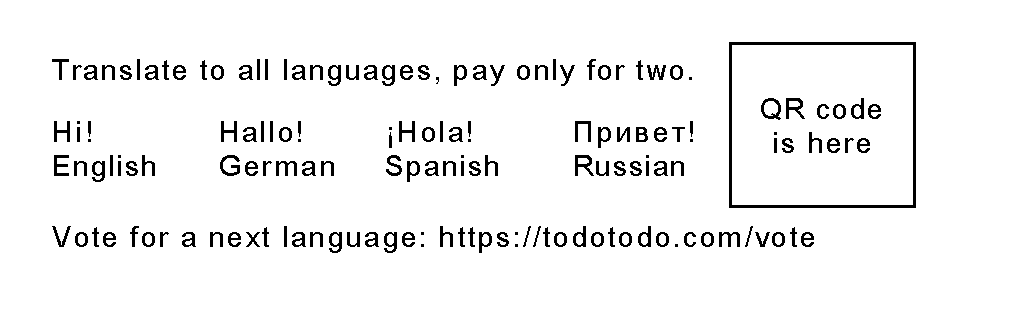
\includegraphics[width=\textwidth]{dia/sample-ad.pdf}}

The voting page asks for the contact information. This way we collect in advance the list of potential clients.

\subsection{Sample request for a meeting}

Slogan in the header: Research -- Prototype -- Business

An: Leiter der technischen Dokumentation

Sehr geehrte Herr Mustermann,

wir haben eine Technologie, die Übersetzungkosten zu senken. Um diese Technologie zur Markt zu bringen, brauchen wir sie anders betrachten, mit den Augen von Kunden. Sie können uns damit helfen. Bitte erzählen Sie uns:

\begin{itemize}
\item welche Hindernisse gibt es, an unsere Technologie zu wechseln
\item davon, welche können wir lösen und welche sind außer unseres Kontrols
\item mit welcher Botschaft sollen wir werben
\end{itemize}

Bitte rufen Sie an -- TODO -- und lade mich zum personlichen Gespräch an. Eine halbe Stunde sollte genug sein.

Mit diesem Gespräch helfen Sie, einen neinen bayerishcen Geschäft auf die Beine zu bringen.

Mit freundlichen Grüßen, Unterschrift

Anlage: über die Technologie. The first sections of this document.


\section{Topics from Leitfragen Executive Summary}

\subsection{Produkt/Dienstleistung}

\paragraph{Was ist Ihre Geschäftsidee?} Language as code to reduce translation costs in multilanguage publishing.

\paragraph{Ist diese Idee einzigartig?}
Yes and no.
\begin{itemize}
\item no: "reduce translation costs" is a big topic
\item yes: the technical approach is unique
\end{itemize}

\paragraph{Was ist das Alleinstellungsmerkmal (USP)?}
The cost is constant regardless the number of target languages.

\paragraph{Ist die Idee geschützt?}
No, and can't be.

\paragraph{Wer sind Ihre Zielkunden?}
Departments of technical documentation of producers of devices, machines, robots.

\paragraph{Was ist der relevante Nutzen für Ihre Zielkunden?}
\begin{itemize}
\item Reduction of translation costs
\item Making the department a lesser cost center
\end{itemize}

\paragraph{Wie ist der aktuelle Entwicklungsstand?}
In a very early stage. See the section \nameref{milestones}.

\paragraph{Welche weiteren Entwicklungsschritte sind erforderlich?}
See the section \nameref{milestones}.

\paragraph{Wie ist die Patentsituation?}
No patents possible.

\paragraph{Welche Pilotkunden haben Sie bzw. können Sie gewinnen?}
We start aquisition as soon as pre-MVP is ready. See the section \nameref{promotion}.

Some former colleagues are now heads of technical documentation departments. They may be interested in doing a test project or providing a reference.

\subsection{Markt und Wettbewerb}
\paragraph{Welches Marktvolumen (Umsatzchancen) und welche Wachstumsrate prognostizieren Sie?}

\paragraph{Welche Wettbewerbssituation liegt vor?}


\subsection{Marketing und Vertrieb}
\paragraph{Welche Markteintrittsstrategie planen Sie?}

\paragraph{Welche Absatzzahlen planen Sie?}

\paragraph{Welche Vertriebskanäle werden Sie nutzen?}


\subsection{Geschäftsmodell und Organisation}
\paragraph{Wie sieht das Geschäftsmodell Ihres Unternehmens aus?}

\paragraph{Welche Partnerschaften wollen Sie eingehen?}

\paragraph{Wie soll Ihre Geschäftsidee organisatorisch umgesetzt werden?}


\subsection{Unternehmerteam, Management, Personal}
\paragraph{Welche Kompetenzen hat das Unternehmerteam und wie verteilen sich die Managementaufgaben?}


\subsection{Realisierungsfahrplan}
\paragraph{Welche langfristigen Ziele haben Sie sich gesetzt?}

\paragraph{Welches sind die wichtigsten Meilensteine auf dem Weg zum Ziel, welche sind schon erreicht?}

\paragraph{Nennen Sie Ihre konkreten nächsten Schritte für die jeweiligen Geschäftsbereiche.}


\subsection{Chancen und Risiken}
\paragraph{Welche Chancen und Risiken bestehen?}


\subsection{Finanzplanung und Finanzierung}
\paragraph{In welcher Höhe müssen Investitionen getätigt werden (Schätzung)?}

\paragraph{Wie ist die Umsatz-, Kosten- und Gewinnsituation?}

\paragraph{Skizzieren Sie die Ergebnisse der detaillierten Geschäftsplanung,}

\paragraph{nennen Sie den exakten Finanzbedarf und die Renditen.}

\paragraph{Woher sollen die Finanzmittel kommen (Finanzierungsquellen)?}


\end{document}
